\chapter{Inspeccionando los datos}
\label{inspeccionando}
En este capítulo se aplicarán distintas técnicas con el objeto de entender en mayor detalle los datos astronómicos con que estamos trabajando, así como descubrir diferentes características del problema de clasificación de RRL. Tener un mayor entendimiento de los datos que se está manipulando puede ayudar a entender por qué RF funciona mejor que SVM.

\section{Importancia de variables}

En esta sección se intentó determinar qué variables son más relevantes a la hora de clasificar RRLs. Para ello se utilizarán:
\begin{itemize}
\item Tests estadísticos univariable, como los utilizados en la sección \ref{filtros_univ}
\item Ranking de importancia asignados por los clasificadores RF y SVM ya entrenados.
\end{itemize} 

Contemplaremos todos los atributos en esta sección, es decir, se omitirá el paso de selección de variables.

\subsection{Tests estadísticos}
Se aplicaron nuevamente tests estadísticos a cada uno de los 62 atributos de los datasets, esta vez con la intención de entender qué variables son más importantes para predecir RRLs.\\

Sea $x_i$ la variable aleatoria que rige el $i-$ésimo atributo de nuestro dataset ($0 \leq i < 62$), discretizado utilizando 100 bins quantile. Por lo tanto, $x_i$ es una variable aleatoria discreta para $0 \leq i < 62$. Sea $y$ la variable aleatoria discreta a predecir, que indica si una dada estrella es RRL o no. \\

Los dos tests estadísticos utilizados analizarán cada atributo $x_i$, planteando el siguiente test de hipótesis \cite{meyer1970introductory}: \\
\begin{adjustwidth}{2cm}{}
\textbf{$H_0$}: La variable $x_i$ es independiente de $y$ \\
\textbf{$H_1$}: La variable $x_i$ no es independiente de $y$ \\
\end{adjustwidth}

Si la hipótesis nula es cierta, entonces $x_i$ es irrelevante por sí misma para predecir $y$. 

\subsubsection{Test $\chi^2$}
El test Pearson $\chi^2$ mide la dependencia entre dos variables estocásticas 
\cite{chi2}. Para explicar intuitivamente cómo funciona, consideremos el clásico dataset Titanic, en el cuál se intenta predecir si un pasajero sobreviviría al hundimiento en base a características como su género, edad y cantidad de familiares en el barco.  \\

Supongamos que deseamos determinar si el atributo género es relevante o no para este problema:

\begin{adjustwidth}{2cm}{}
\textbf{$H_0$}: El atributo género es independiente de la supervivencia de un pasajero. \\
\textbf{$H_1$}: El atributo género no es independiente de la supervivencia de un pasajero. \\
\end{adjustwidth}

Con una simple visualización de los datos, como la mostrada en la figura \ref{fig:chi2_titanic}, podemos apreciar que la proporción de hombres y mujeres no es la misma para sobrevivientes que para no sobrevivientes. Esto nos indica, intuitivamente, que el género de una persona es ciertamente informativo para predecir la supervivencia de un pasajero. En la figura \ref{fig:chi2_titanic_freq} (a) podemos ver estas frecuencias en una matriz de confusión. 

\begin{figure}[h!]
\centering
  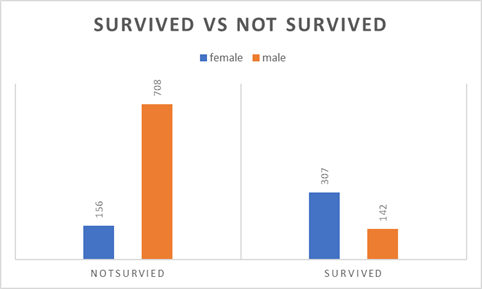
\includegraphics[width=0.49\textwidth]{Kap6/chi2titanic.png}
\caption{ Supervivencia de pasajeros del Titanic discriminada por género. Créditos: Dr. Saptarsi Goswami }
\label{fig:chi2_titanic}
\end{figure}


\begin{figure}[h!]
\begin{tabular}{cc}

\begin{tabular}{|l|l|l|l|}
\hline
                    & \textbf{No Sobrev} & \textbf{Sobrev} & total \\ \hline
\textbf{Mujer}      & 156              & 307             & 463    \\ \hline
\textbf{Hombre}     & 708              & 142             & 850    \\ \hline
total               & 864              & 449             & 1313   \\ \hline
\end{tabular}


 &   
 
 \begin{tabular}{|l|l|l|l|}
\hline
                    & \textbf{No Sobrev} & \textbf{Sobrev} & total \\ \hline
\textbf{Mujer}      & 304,67           & 158.33          & 463    \\ \hline
\textbf{Hombre}     & 559.33              & 290.67             & 850    \\ \hline
total               & 864              & 449             & 1313   \\ \hline
\end{tabular}
 \\
(a) Frecuencias observadas & (b) Frecuencias esperadas
\end{tabular}
\caption{Frecuencias en el dataset Titanic. Hay $n=1313$ personas en este dataset.}
\label{fig:chi2_titanic_freq}
\end{figure}


Por otro lado, asumiendo que la hipótesis nula (independencia) es cierta, la siguiente igualdad vale:

\begin{center}
 $P(genero \wedge sobrevivio) = P(genero) * P(sobrevivio)$
\end{center}
 
Bajo esta asunción, se puede calcular la tabla de  \textbf{frecuencias esperadas} de la figura \ref{fig:chi2_titanic_freq} (b). Por ejemplo, para la primera celda, correspondiente a cuántas mujeres no sobrevivieron:

\begin{align*}
  E_1 & = n   * P(genero=Mujer \wedge sobrevivio=NoSobrevivio) \\
      & = n   * P(genero=Mujer) * P(sobrevivio=NoSobrevivio) \\
      & = 1313 * \frac{463}{1313} * \frac{864}{1313} \\
      & = 304.67
\end{align*}

Si la hipótesis nula fuese cierta, las frecuencias de las dos tablas de la figura \ref{fig:chi2_titanic_freq} deberían ser iguales celda a celda. $\chi^2$ mide la disparidad entre ambas, y se define como sigue:

\begin{center}
$\chi^2 = \sum_i \frac{(O_i - E_i)^2}{E_i}$
\end{center}

Donde $O_i$ y $E_i$ son la frecuencia observada y esperada para la $i$-ésima entrada de la tabla de confusión de las variables a testear. En la siguiente tabla podemos ver cómo se calcula el valor $\chi^2 = 327.7$ para nuestro ejemplo:

\begin{table}[h!]
\center
\begin{tabular}{|l|l|l|l|l|}
\hline
\textbf{Género}  & \textbf{Sobrevivió}    & $O_i$   & $E_i$    &  $\frac{ (O-E)^2 }{E}$ \\ \hline
Mujer   & Sí    & 307     & 158.33   &  139.59                \\ \hline
Mujer   & No  & 156     & 304.67   &  72.54                 \\ \hline
Hombre  & Sí    & 142     & 290.77   &  76.04                 \\ \hline
Hombre  & No  & 708     & 559.33   &  39.51                 \\ \hline
$\chi^2$ value &   &    &         &           327.70                \\ \hline
\end{tabular}
\end{table}

El valor $\chi^2$ puede ser interpretado para decidir si rechazar o aceptar la hipótesis nula, donde un mayor valor de $\chi^2$ indica evidencia en contra de la hipótesis nula. La interpretación se realiza calculando el p-value correspondiente al valor de $\chi^2$ obtenido\footnote{La correspondencia entre $\chi^2$ y p-values suele estar tabulada, pues es bastante compleja de calcular.}, que en conjunto con un nivel de significación $\alpha$ deseado puede interpretarse como: 

\begin{itemize}
\item p-value $\leq \alpha$: Rechazar $H_0$, las variables son dependientes.
\item p-value $> \alpha$: No rechazar $H_0$,  las variables son independientes.
\end{itemize}

Para nuestro ejemplo, la diferencia entre las tablas es tan grande que el p-value asociado es $\sim0$, por lo que la hipótesis nula es rechazada. El género de una persona es importante a la hora de predecir si sobrevivió o no. Aplicaremos este test estadístico a los atributos de los datasets de Carpyncho en la sección \ref{experimentos_test_estadisticos}. \\

\subsubsection{ANOVA F test}
\label{f_test}
ANOVA (ANalysis Of VAriance) es un método estadístico utilizado para chequear si la media de dos o más grupos de datos son significativamente diferentes \cite{191611} \cite{han2012mining}. Las hipótesis son:\\

\begin{adjustwidth}{2cm}{}
\textbf{$H_0$}: Las medias de todos los grupos son iguales. \\
\textbf{$H_1$}: Al menos la media de uno de los grupos es distinta. \\
\end{adjustwidth}

El resultado del test es una medida estadística, F score, que es inversamente proporcional al p-value asociado al test estadístico. \\

ANOVA puede ser utilizado para decidir si un cierto atributo de un dataset es relevante o no para predecir una variable objetivo. La figura \ref{fig:anova_example} provee un ejemplo ilustrativo: se presenta un dataset con dos atributos $x_1$ (horizontal) y $x_2$ (vertical),  en tanto que la variable a predecir $y$ está demarcada con colores (rojo y azul). Se desea asignar un puntaje a cada atributo indicando cuán bien cada uno discrimina entre rojos y azules. \\

Al proyectar los elementos de cada color por separado en cada eje, podemos apreciar que $x_1$ es mucho mejor separando las clases que $x_2$, por dos motivos:

\begin{itemize}
\item Las medias de las distribuciones de probabilidad proyectadas están más separadas.
\item Las distribuciones de probabilidad proyectadas son más compactas.
\end{itemize}

Estas dos cualidades son exactamente lo que el test ANOVA mide, numéricamente, para cada atributo. Como resultado, obtendremos un F score para cada atributo. El F score de $x_1$ será mayor que el F score asignado a $x_2$. Finalmente, el F-score de cada variable podrá ser convertido a un p-value para decidir si la hipótesis nula del test ANOVA puede ser rechazada o no. Si la hipótesis nula es rechazada, se puede concluir que el atributo en cuestión es relevante a la hora de predecir $y$. 
%http://www.thesiliconboard.com/page/3/

\begin{figure}[h!]
\centering
  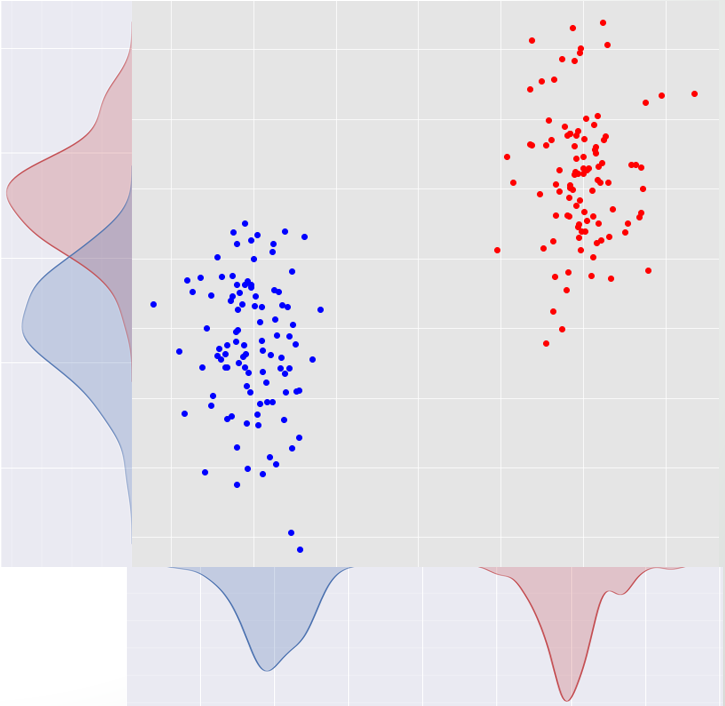
\includegraphics[width=0.6\textwidth]{Kap6/anova_example.png}
\caption{ Ejemplo de ANOVA F-value test. Créditos: Kasra Manshaei }
\label{fig:anova_example}
\end{figure}

\subsubsection{Experimentos con tests estadísticos}
\label{experimentos_test_estadisticos}
Habiendo introducido brevemente los dos tests estadísticos que se utilizaron, se procederá a reportar los resultados de aplicar ambos tests a cada uno de los 62 atributos utilizados por Carpyncho para describir estrellas RRL. En la figura \ref{fig:pvalues_b278} podemos ver los p-values obtenidos por ambos tests para cada atributo del dataset \textit{b278}. Gráficas similares para \textit{b234}, \textit{b360} y \textit{b261} se encuentran en el anexo \ref{anexo_b_pvalues}. \\

Recordemos que altos p-values indican mayor evidencia a favor de la hipótesis nula. Es decir, altos p-values indican independencia entre el atributo en cuestión y la variable objetivo, por lo tanto tales atributos son considerados irrelevantes para detectar RRLs por si mismos. Tomando un nivel de significación $\alpha=0.05$, los siguientes atributos son consistentemente clasificados como irrelevantes de acuerdo a ANOVA:

\begin{itemize}
\item Freq1\_harmonics\_rel\_phase\_1, Freq1\_harmonics\_rel\_phase\_2, Freq1\_harmonics\_rel\_phase\_3 

\item Freq2\_harmonics\_rel\_phase\_1, Freq2\_harmonics\_rel\_phase\_2, Freq2\_harmonics\_rel\_phase\_3

\item Freq3\_harmonics\_rel\_phase\_1, Freq3\_harmonics\_rel\_phase\_2, Freq3\_harmonics\_rel\_phase\_3
\item Amplitude
\item LinearTrend
\item PairSlopeTrend
\end{itemize}


Utilizando el mismo nivel de significación, $\chi^2$ parece ser un poco más conservador a la hora de declarar atributos como irrelevantes. Más aún, las conclusiones extraídas por $\chi^2$ no son completamente consistentes entre distintos tiles. Los siguientes atributos son declarados como irrelevantes en la mayoría de los tiles:

\begin{itemize}
\item Freq1\_harmonics\_rel\_phase\_1, Freq1\_harmonics\_rel\_phase\_2
\item Freq2\_harmonics\_amplitude\_phase\_2
\item Freq2\_harmonics\_rel\_phase\_2, Freq2\_harmonics\_rel\_phase\_3
\item Freq3\_harmonics\_rel\_phase\_1, Freq3\_harmonics\_rel\_phase\_2
\item PairSlopeTrend
\end{itemize}

Podemos ver que ambos tests coinciden en que varios de los atributos que describen las componentes de Fourier parecen ser irrelevantes a la hora de diferenciar RRLs. Estos atributos están entre los primeros en ser eliminados en los experimentos de selección de variables (ver sección \ref{filtros_univ}) que se realizaron en el capítulo anterior, y se ha verificado que eliminarlos no reduce performance, de hecho la mejora en SVM-RBF. \\

\begin{figure}[h!]
\centering
  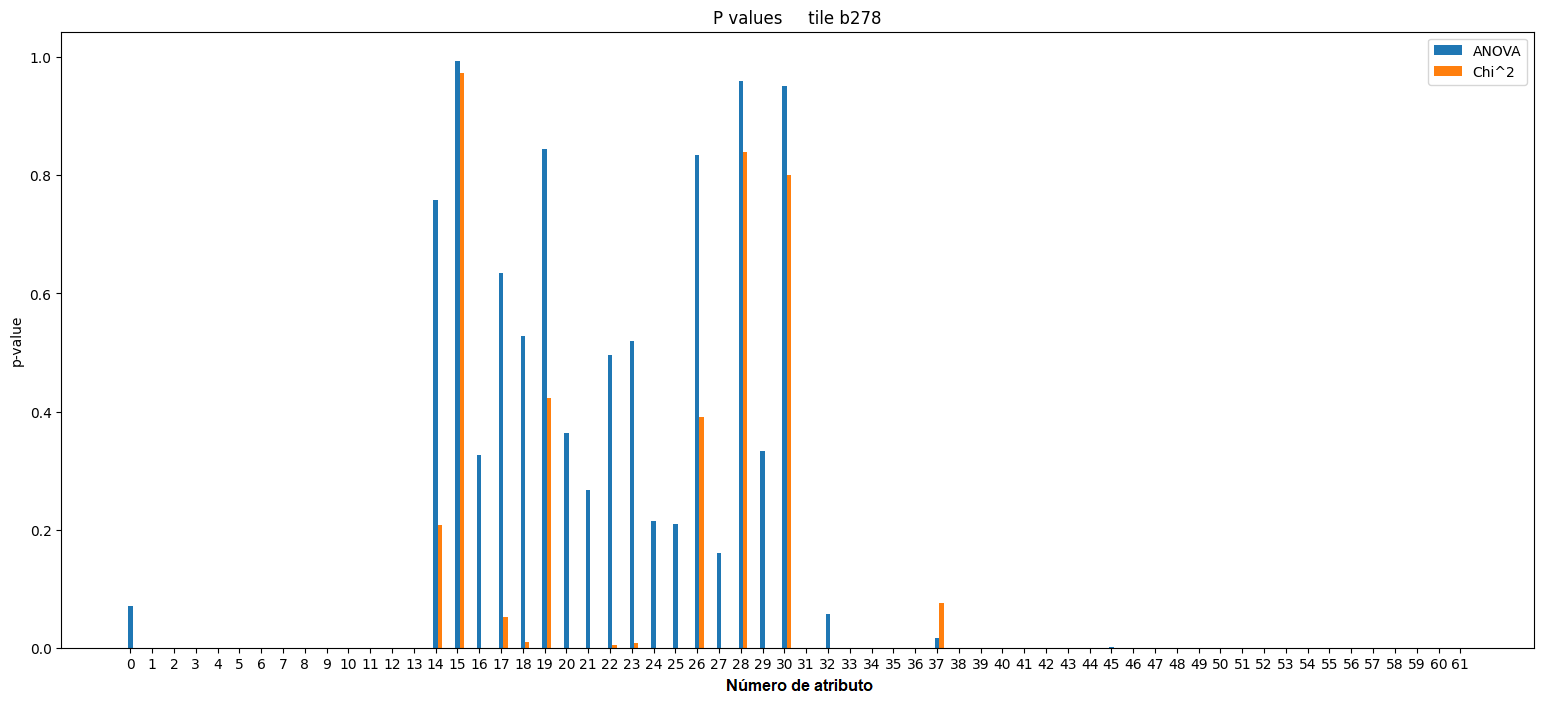
\includegraphics[width=1\textwidth]{Kap6/test=b278_variable_importance_pvalues}
\caption{ p-values resultantes de los tests estadísticos ANOVA y $\chi^2$ aplicados a cada atributo del tile b278. En el anexo \protect\ref{indice_atributos} puede consultarse la lista completa de atributos. }
\label{fig:pvalues_b278}
\end{figure}

Por otro lado, si se desea estudiar qué atributos son más importantes, podemos inspeccionar cuáles de ellos maximizan las métricas $\chi^2$, F-score e información mutua (ver sección \ref{filtros_univ}). Nótese que, a diferencia de los p-values, estas métricas no se encuentran en una misma escala; y los valores absolutos obtenidos no son directamente comparables entre sí. \\

En la figura \ref{fig:scores_b278} se presentan las métricas para cada atributo en b278, unificadas en una misma gráfica. Cada métrica fue normalizada de forma tal que la sumatoria de los puntajes en todos los atributos es 1. Gráficas similares para \textit{b234}, \textit{b360} y \textit{b261} se encuentran en el anexo \ref{anexo_b_scores}. \\

En la práctica, la forma de utilizar estos puntajes muchas veces consiste en seleccionar los $k$ atributos que maximizan la métrica utilizada. En este contexto, los valores absolutos de los puntajes no son relevantes, y resulta más informativo considerar la posición en el ranking que cada atributo recibe. Esto puede visualizarse en la figura \ref{fig:ranking_b278}, en tanto que las gráficas correspondients a \textit{b234}, \textit{b360} y \textit{b261} se encuentran en el anexo \ref{anexo_b_rankings}. 

\begin{itemize}
\item En primer lugar, veamos que mutual information presenta poca variación en sus puntajes, a excepción de cuatro atributos que son consistentemente destacados: Autocolor\_length, Beyond1Std, PairSlopeTrend y Period\_fit.
\item El F-score destaca consistentemente los atributos Autocolor\_length y Period\_fit. También reciben puntajes considerables los atributos FluxPercentile y las primeras componentes de fourier, así como los índices Psi\_CS y Psi\_eta y algunos atributos de color.
\item $\chi^2$ destaca Psi\_CS, Psi\_eta, así como algunos atributos de color (51 52 57 58), FluxPercentile, las primeras componentes de Fourier, y Period\_fit.
\end{itemize}


\begin{figure}[h!]
\centering
  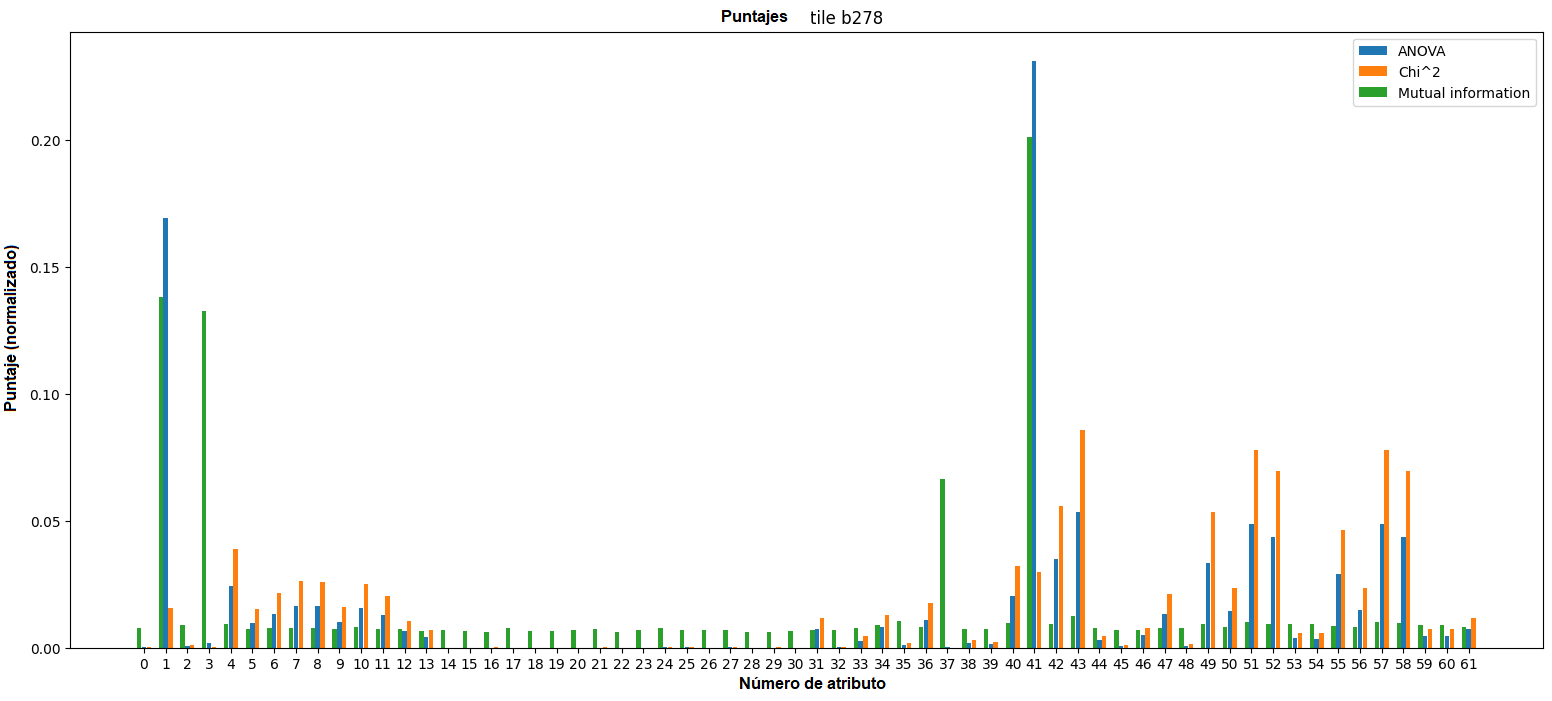
\includegraphics[width=1\textwidth]{Kap6/test=b278_variable_importance_scores}
\caption{ Métricas $\chi^2$, ANOVA F-score e información mutua calculadas para cada atributo del tile b278. En el anexo \protect\ref{indice_atributos} puede consultarse la lista completa de atributos. }
\label{fig:scores_b278}
\end{figure}

\begin{figure}[h!]
\centering
  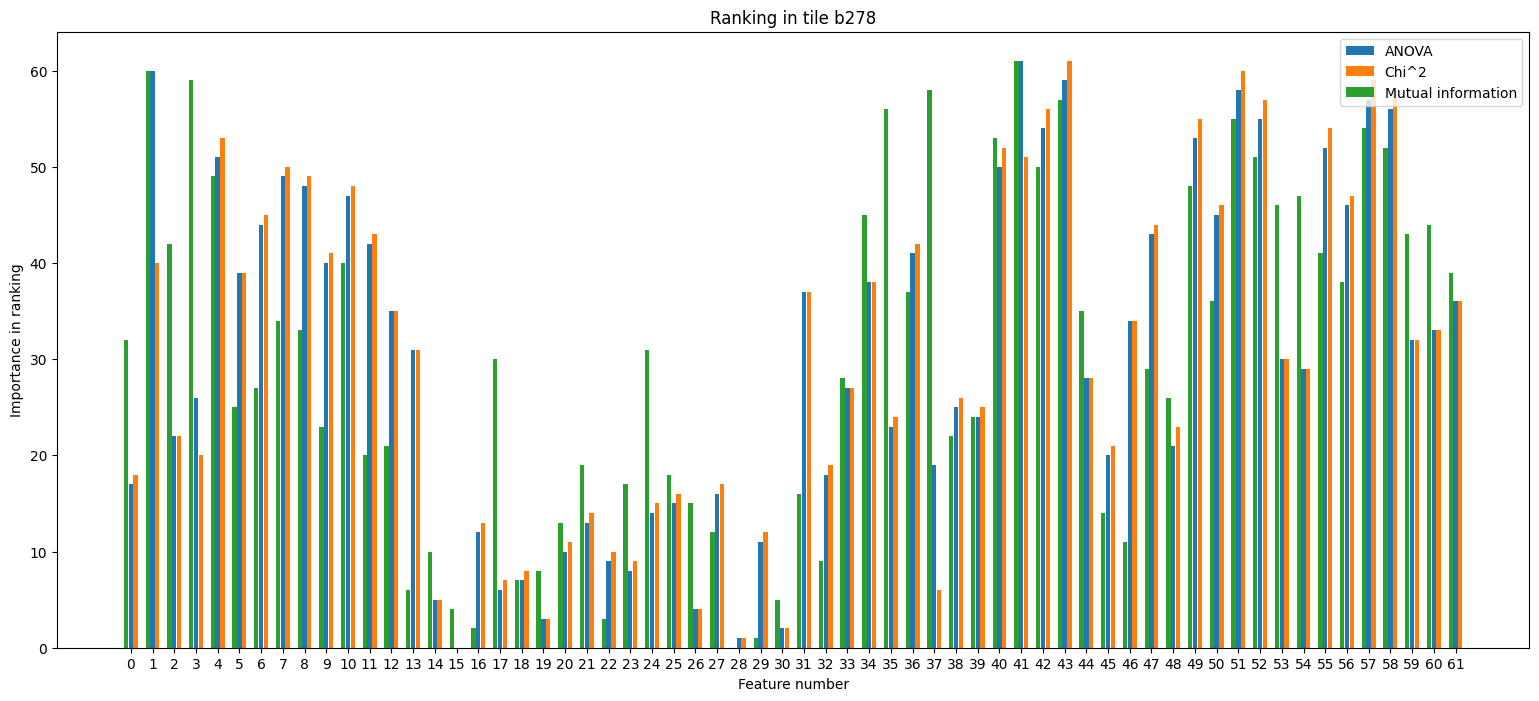
\includegraphics[width=1\textwidth]{Kap6/test=b278_variable_importance_ranking}
\caption{ Ranking de variables obtenido por las métricas $\chi^2$, ANOVA F-score e información mutua calculadas para cada atributo del tile b278. En el anexo \protect\ref{indice_atributos} puede consultarse la lista completa de atributos. }
\label{fig:ranking_b278}
\end{figure}

\subsection{Importancia basada en clasificadores}

Los clasificadores RF pueden proveer un puntaje (importancia) a cada atributo del dataset de entrenamiento, llamado importancia Gini (o reducción media en impuridad, MDI) \cite{statisticallearning}. Para cada atributo, este valor se calcula como la cantidad de veces que ese atributo se utiliza como criterio de división en un nodo (en todos los árboles), ponderado por la cantidad de instancias que ese nodo divide. \\

Por otro lado, luego de entrenar SVM con kernel lineal, podemos inspeccionar el valor absoluto del vector de pesos $w$ para comprender cuánta importancia SVM le asigna a cada atributo \cite{svm_importance}. Esto no es posible para SVM RBF pues los datos son transformados a otro espacio, por lo tanto el plano separador existe en otro espacio y los coeficientes no tienen una relación trivial con los atributos del espacio original. \\

En la figura \ref{fig:ml_importance_b278} podemos ver la importancia (normalizada) que SVM-Lineal y RF asignan a cada atributo en el tile b278. Las gráficas para los tiles restantes se encuentran en el anexo \ref{anexo_ml_scores}. \\

\begin{figure}[h!]
\centering
  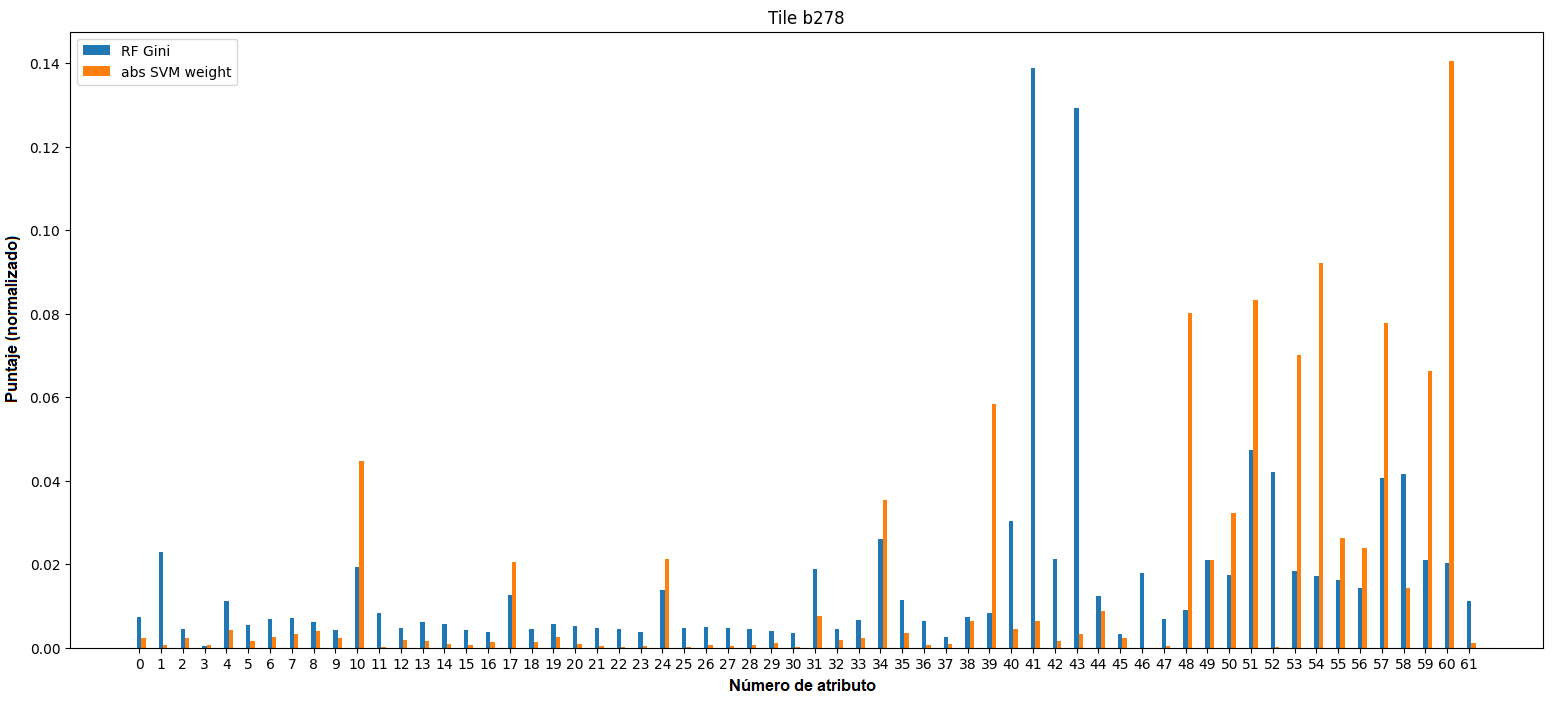
\includegraphics[width=1\textwidth]{Kap6/test=b278_ML_variable_importance_scores}
\caption{ Importancia asignada por RF y SVM-Lineal a cada atributo del tile b278. En el anexo \protect\ref{indice_atributos} puede consultarse la lista completa de atributos. }
\label{fig:ml_importance_b278}
\end{figure}

Los rankings de variables generados por Random Forest son muy consistentes entre distintos tiles. Se puede observar que:

\begin{itemize}
\item La variable más importante es \textbf{PeriodFit} seguida por \textbf{Psi\_eta}. Nótese que tanto ANOVA como mutual information consistentemente colocaban a PeriodFit como el atributo más importante y a Psi\_eta entre los 5 más importantes. Por otro lado, el ranking de $\chi^2$ posiciona a Psi\_eta con la máxima importancia pero en algunos tiles fallaba en detectar la verdadera importancia de PeriodFit.
\item Con aproximadamente la mitad de importancia que las dos variables recién mencionadas, RF también considera importantes a Psi\_CS, c89\_jh\_color y c89\_jk\_color, n\_09\_jh\_color y n\_09\_jk\_color, y Autocor\_length. Con distintos grados de precisión, los tests estadísticos efectivamente marcan a estos atributos como relevantes para detectar RRLs.
\end{itemize}

Por otro lado, luego de analizar a qué variables SVM-Lineal está ponderando, podemos observar que se está prestando alta atención a las variables de color (48 a 60). Se puede también observar que SVM ignora atributos clave como PeriodFit y Psi\_eta que, como ya hemos validado a través de tests estadísticos e importancia gini, son altamente informativos para detectar RRLs. \\

\section{ Análisis de correlaciones }

\subsection{ Correlación entre atributos }

En esta sección nos concentraremos en entender las distintas correlaciones presentes entre los atributos de nuestros datasets, sin tener en cuenta la variable a predecir. Para ello, se computó un coeficiente de correlación en $[-1,1]$ para cada par de atributos, que mide cuán fuertemente correlacionado cada par está. Un valor de $\pm 1$ indica un grado de asociación perfecto entre las variables, en tanto que valores cercanos a $0$ indican una relación más débil. El signo indica si la relación es directa o inversa.  \\

A la hora de realizar tales cálculos, es muy importante utilizar una métrica de correlación adecuada \cite{how_to_choose_correlation}. Por ejemplo, la métrica más comúnmente utilizada, el coeficiente de correlación de Pearson \cite{pagano2010understanding}, sería inadecuada para nuestros atributos, dado que requiere que ambos atributos estén distribuidos de forma normal y sean continuos. \\

Dado que nuestros atributos (luego de binning) son de tipo discretos ordinales (con a lo sumo ~100 valores ordenados), resulta apropiado el uso de ténicas que midan la semejanza de ordenamientos (o rankings) de los datos  \cite{how_to_choose_correlation} \cite{pagano2010understanding}, tales como el \textbf{Coeficiente de correlación de rango de Kendall} ($\tau$, \cite{kendall_spearman}) y el \textbf{Coeficiente de correlación de rango de Spearman} ($\rho$, \cite{kendall_spearman}) \\

Tanto $\rho$ como $\tau$ son capaces de medir correlaciones monotónicas arbitrarias, a diferencia del coeficiente de Pearson que es únicamente capaz de medir correlaciones lineares \cite{pagano2010understanding}. En la figura \ref{fig:correlation_matrix_b278_sp} podemos ver la matriz de correlación utilizando el coeficiente de Spearman, en tanto que en la figura \ref{fig:correlation_matrix_b278_ke} podemos ver la matriz de correlación de acuerdo al coeficiente de Kendall. Las matrices de correlación de los tiles restantes se encuentran en el anexo \ref{anexo_matrices_correlacion}. \\

\begin{figure}[h!]
\centering
  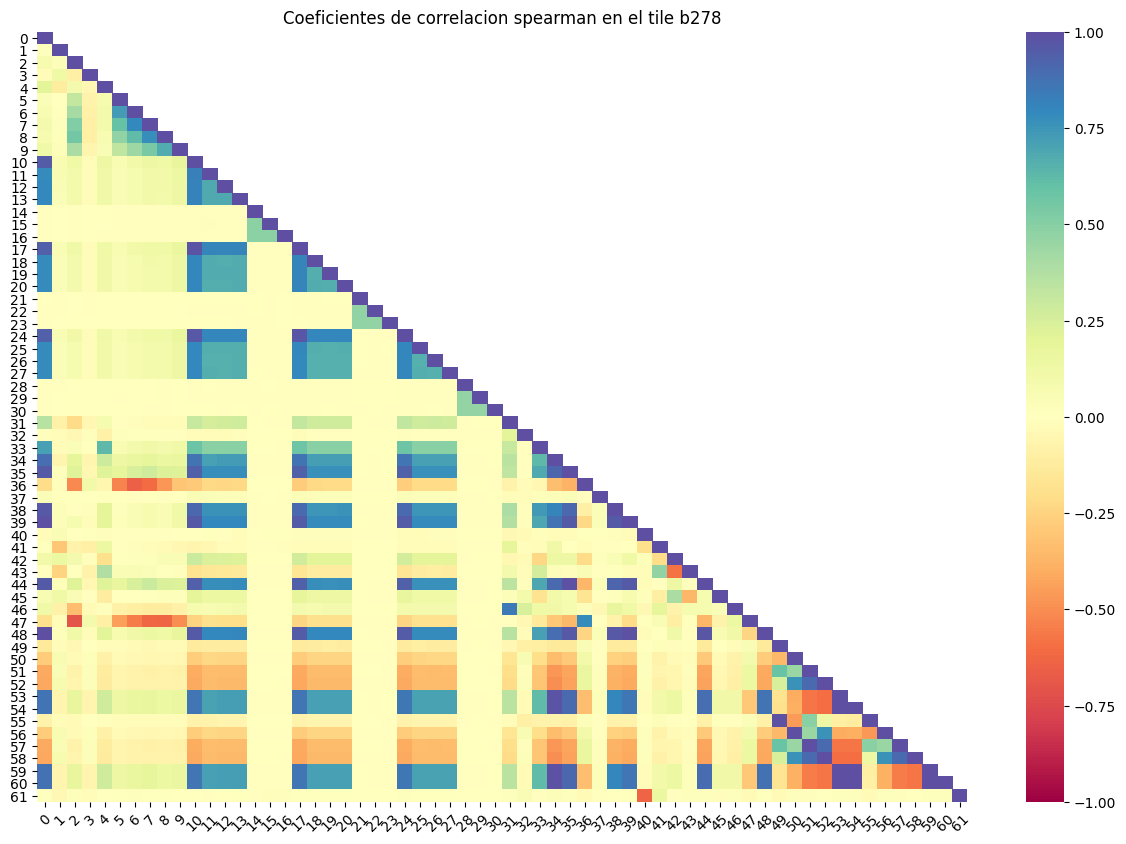
\includegraphics[width=1\textwidth]{Kap6/spearman_b278_MATRIX.png}
\caption{ Correlaciones lineales (métrica de Spearman) en el tile b278. En el anexo \protect\ref{indice_atributos} puede consultarse la lista completa de atributos. }
\label{fig:correlation_matrix_b278_sp}
\end{figure}

\begin{figure}[h!]
\centering
  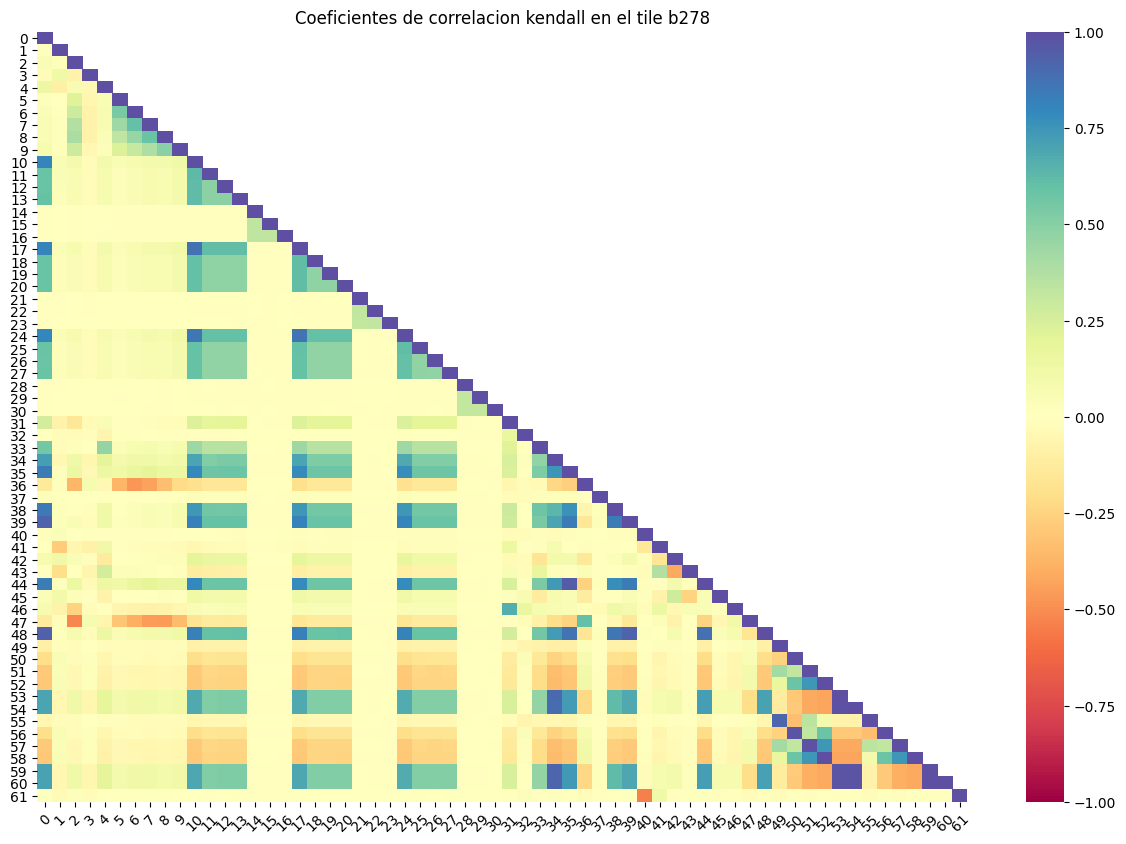
\includegraphics[width=1\textwidth]{Kap6/kendall_b278_MATRIX.png}
\caption{ Correlaciones lineales (métrica de Kendall) en el tile b278. En el anexo \protect\ref{indice_atributos} puede consultarse la lista completa de atributos. }
\label{fig:correlation_matrix_b278_ke}
\end{figure}


Podemos observar que los coeficientes de correlación son bastante consistentes entre distintos tiles para ambos métodos. Ambos métodos, $\tau$ y $\rho$, identifican los mismos grupos de atributos como correlacionados; aunque los valores absolutos de correlación obtenidos por $\tau$ son ligeramente menores. Este fenómeno es esperable, dado que $\tau$ tiende a producir valores absolutos más pequeños que $\rho$. \\

Los bloques de atributos correlacionados más prominentes son:

\begin{itemize}
\item Los \textbf{atributos de color} (49 a 60) están, naturalmente, altamente correlacionados entre sí. Podemos notarlo porque la esquina inferior derecha de la matriz muestra altos valores entre la mayoría de los pares; así como con los atributos \textbf{Mean} y \textbf{Amplitude}.
\item Los atributos \textbf{Amplitude}, \textbf{MedianAbsDev}, \textbf{PercentAmplitude}, \textbf{PercentDifferenceFluxPercentile}, \textbf{Q31} y \textbf{Std} tienden a estar altamente correlacionados entre sí. Esto es esperable, dado que todos estos atributos son estadísticas descriptivas calculadas a partir de las magnitudes observadas.
\item \textbf{Beyond1Std}, \textbf{SmallKurtosis} y \textbf{MedianBRP}
\item Naturalmente, los atributos \textbf{FluxPercentileRatioMid\_\textit{x}} para $x=20, 35, 50, 65, 80$ exponen una leve correlación. Esta correlación no es tan fuerte, lo cuál indica que estos atributos contienen información ligeramente distinta.
\item Los atributos que describen las amplitudes de las primeras tres componentes de Fourier de los tres primeros períodos candidatos (atributos 10-13, 17-20 y 24-27) están todos correlacionados entre sí. Esto indica que los primeros tres períodos candidatos de cada RRL son similares en amplitud.
\end{itemize}

Numéricamente, algunas de las correlaciones son extremadamente fuertes, alcanzando valores absolutos mayores a 0.99, lo cuál indica que ciertos pares de variables contienen información completamente redundante.

\subsection{ Eliminación de atributos correlacionados }

En esta sección se analizó si eliminar atributos altamente correlacionados trae algún beneficio interesante en las curvas de precision-recall obtenidas utilizando SVM. Para ello, se realizó el siguiente experimento dado un tile de entrenamiento y un tile de testing:

\begin{enumerate}
\item Calcular la matriz de correlaciones de Spearman en el dataset de entrenamiento.
\item Identificar el par de atributos tal que el valor absoluto de su coeficiente de correlación es máximo.
\item Seleccionar un atributo del par, y eliminarlo del dataset de entrenamiento y de test
\item Entrenar SVM utilizando el dataset de training resultante, y calcular el R-AUPRC en test.
\item Repetir (1) hasta que no queden más atributos.
\end{enumerate}

En las figuras \ref{fig:svml_correlation_remove} (SVM-L) y \ref{fig:svmk_correlation_remove} (SVM-RBF) podemos ver el efecto R-AUPRC obtenido cada vez que se elimina el atributo más correlacionado restante, así como la base de referencia obtenido en la sección \ref{baseline_preproc}.

\begin{figure}[h!]
\begin{tabular}{cccc}
  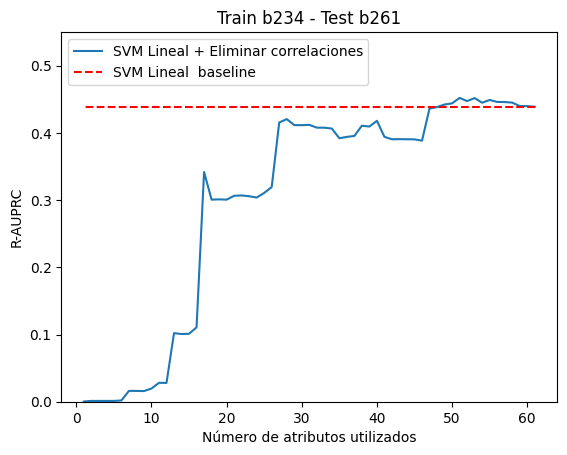
\includegraphics[width=0.25\textwidth]{Kap6/pearson_linear_INDIVIDUAL_CURVES_train=b234test=b261}  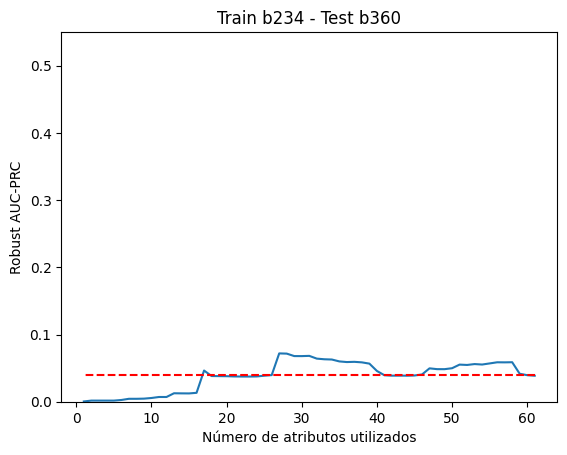
\includegraphics[width=0.25\textwidth]{Kap6/pearson_linear_INDIVIDUAL_CURVES_train=b234test=b360}
  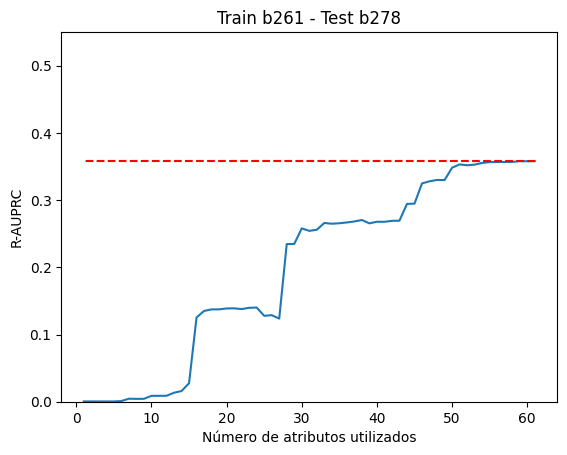
\includegraphics[width=0.25\textwidth]{Kap6/pearson_linear_INDIVIDUAL_CURVES_train=b261test=b278}  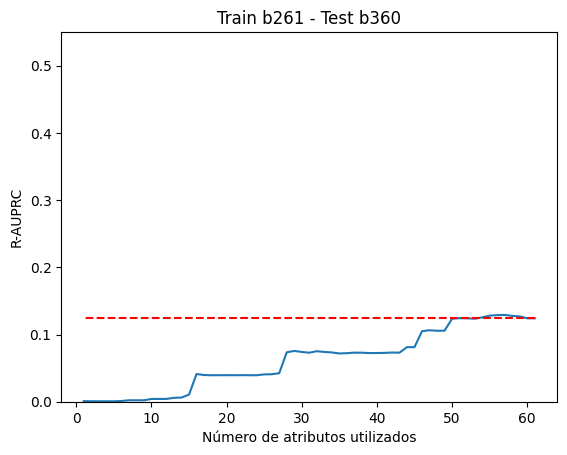
\includegraphics[width=0.25\textwidth]{Kap6/pearson_linear_INDIVIDUAL_CURVES_train=b261test=b360} \\

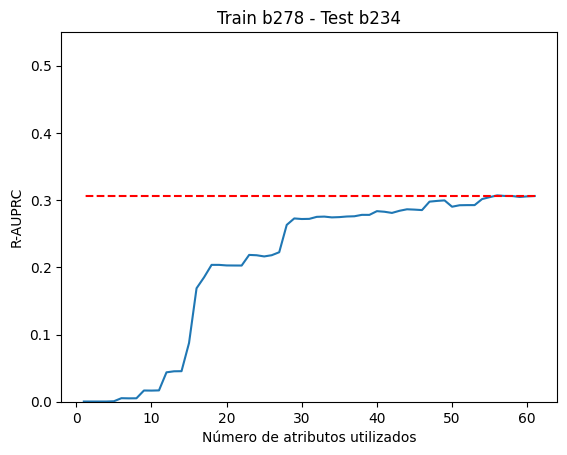
\includegraphics[width=0.25\textwidth]{Kap6/pearson_linear_INDIVIDUAL_CURVES_train=b278test=b234}  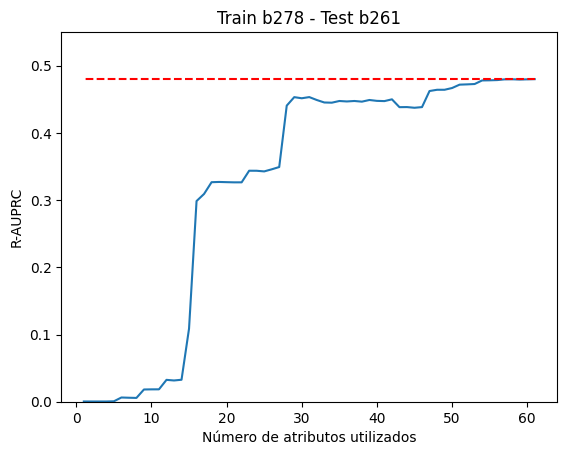
\includegraphics[width=0.25\textwidth]{Kap6/pearson_linear_INDIVIDUAL_CURVES_train=b278test=b261} 
 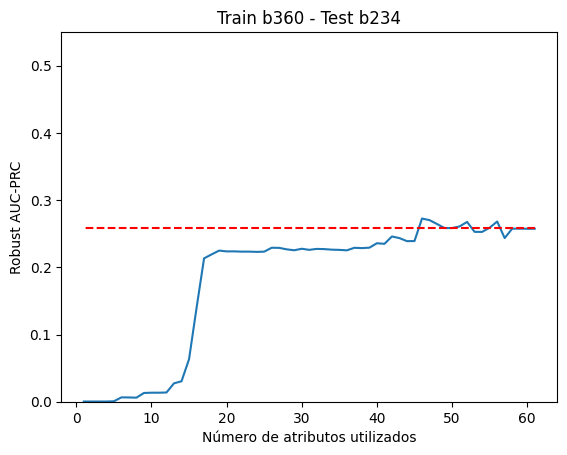
\includegraphics[width=0.25\textwidth]{Kap6/pearson_linear_INDIVIDUAL_CURVES_train=b360test=b234}  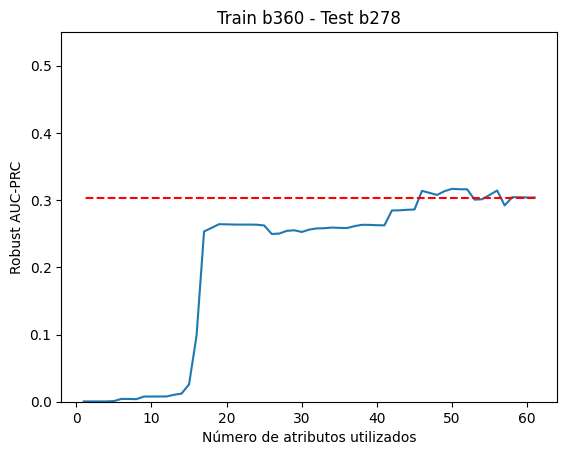
\includegraphics[width=0.25\textwidth]{Kap6/pearson_linear_INDIVIDUAL_CURVES_train=b360test=b278} 
\end{tabular}
\caption{Efecto de eliminar atributos altamente correlacionados en SVM Lineal}
\label{fig:svml_correlation_remove}
\end{figure}

\begin{figure}[h!]
\begin{tabular}{cccc}
  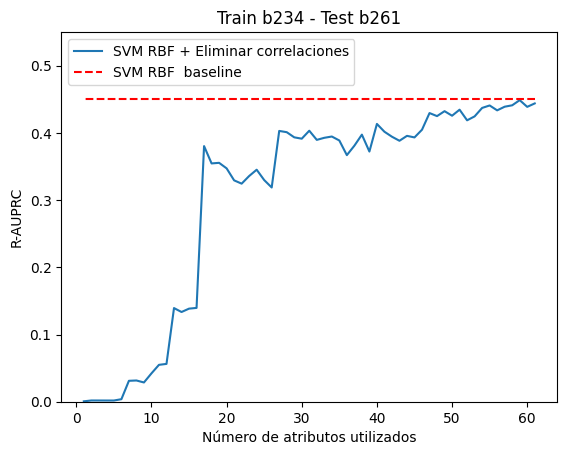
\includegraphics[width=0.25\textwidth]{Kap6/pearson_rbf_INDIVIDUAL_CURVES_train=b234test=b261}  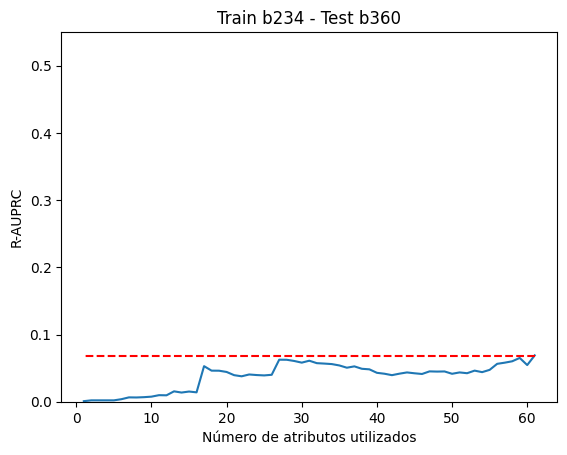
\includegraphics[width=0.25\textwidth]{Kap6/pearson_rbf_INDIVIDUAL_CURVES_train=b234test=b360}
  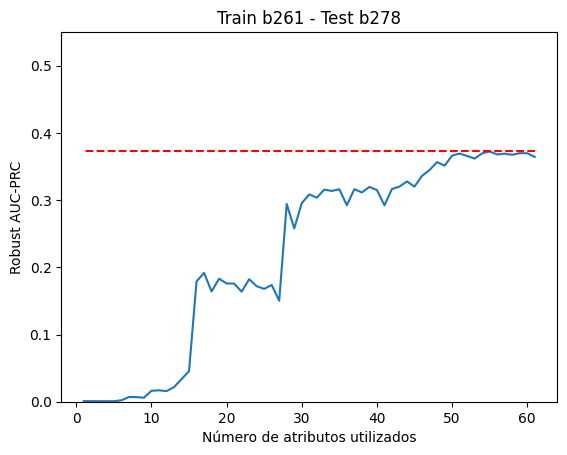
\includegraphics[width=0.25\textwidth]{Kap6/pearson_rbf_INDIVIDUAL_CURVES_train=b261test=b278}  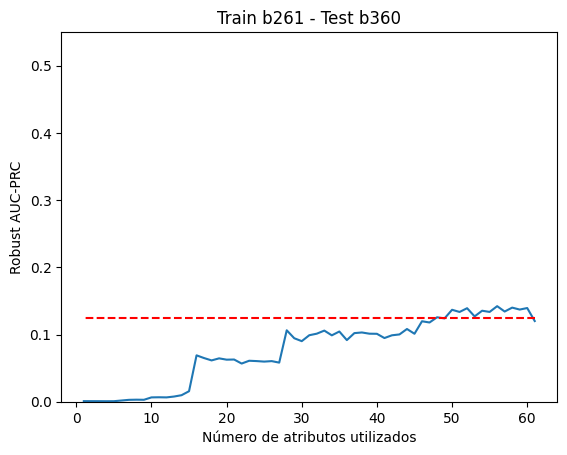
\includegraphics[width=0.25\textwidth]{Kap6/pearson_rbf_INDIVIDUAL_CURVES_train=b261test=b360} \\

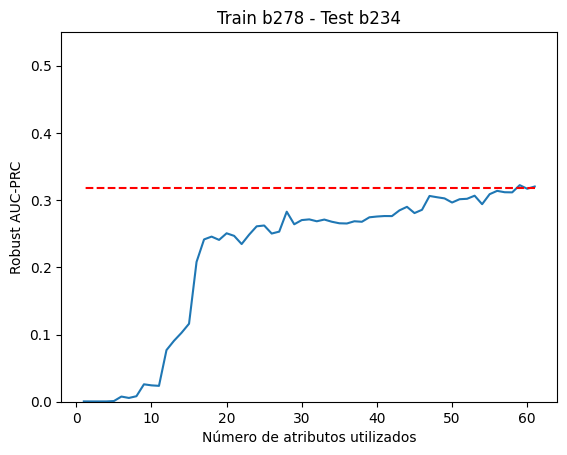
\includegraphics[width=0.25\textwidth]{Kap6/pearson_rbf_INDIVIDUAL_CURVES_train=b278test=b234}  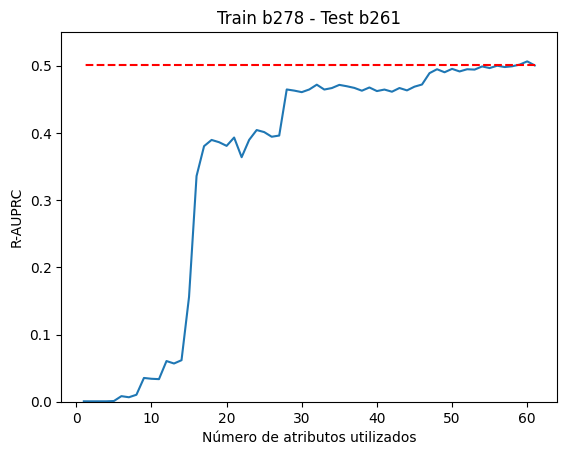
\includegraphics[width=0.25\textwidth]{Kap6/pearson_rbf_INDIVIDUAL_CURVES_train=b278test=b261} 
 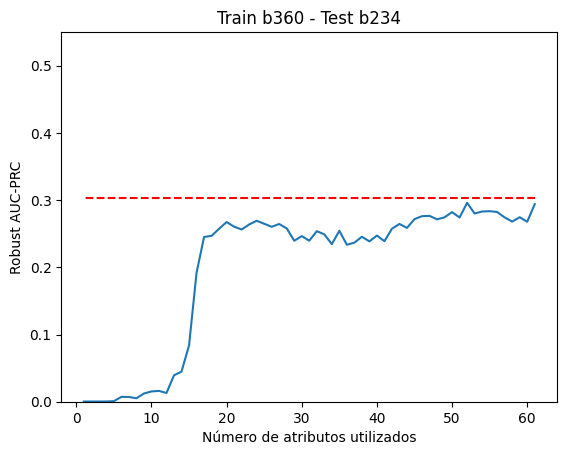
\includegraphics[width=0.25\textwidth]{Kap6/pearson_rbf_INDIVIDUAL_CURVES_train=b360test=b234}  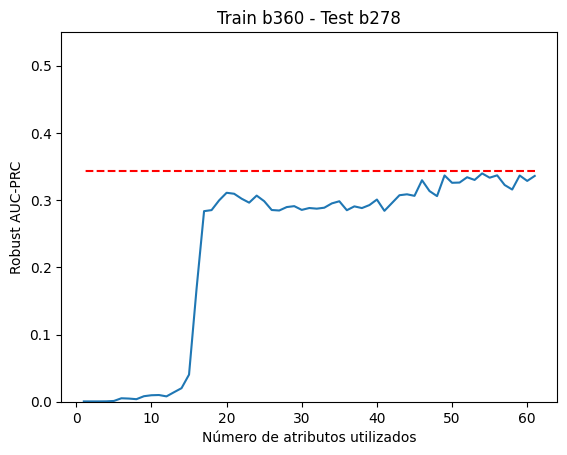
\includegraphics[width=0.25\textwidth]{Kap6/pearson_rbf_INDIVIDUAL_CURVES_train=b360test=b278} 
\end{tabular}
\caption{Efecto de eliminar atributos altamente correlacionados en SVM RBF}
\label{fig:svmk_correlation_remove}
\end{figure}

Para resumir la información de las figuras \ref{fig:svml_correlation_remove} y \ref{fig:svmk_correlation_remove}, se calculó la distancia promedio y mínima a la base de referencia de todos los tiles. Estos cálculos están graficados en la figura \ref{fig:svm_correlation_summary}, y nos permiten concluir que:

\begin{itemize}
\item  En SVM Lineal, eliminar atributos altamente correlacionados no nos permite mejorar (en promedio) las curvas de precision-recall respecto a la base de referencia. Esto es válido incluso si nos remitimos a eliminar únicamente aquellos que muestran una correlación muy fuerte.
\item Si bien no hay mejora en las curvas de precision-recall, en SVM Lineal podemos eliminar los primeros $\sim17$ atributos más correlacionados sin provocar pérdida de R-AUPRC en promedio. Esto indica que los atributos altamente correlacionados no contienen información vital para SVM-Lineal.
\item A diferencia de SVM-Lineal, la performance de SVM-RBF se ve perjudicada al eliminar incluso los atributos con mayor coeficiente de correlación. 
\end{itemize}

Como conclusión de esta sección, podemos decir que la existencia de atributos altamente correlacionados no tiene un impacto negativo en la performance de los clasificadores SVM. De hecho, prescindir de los atributos más correlacionados no mejora en absoluto la performance de los clasificadores estudiados. Las correlaciones entre variables no son el motivo por el cuál SVM funciona peor que RF.

\begin{figure}[h!]
\begin{tabular}{cc}
  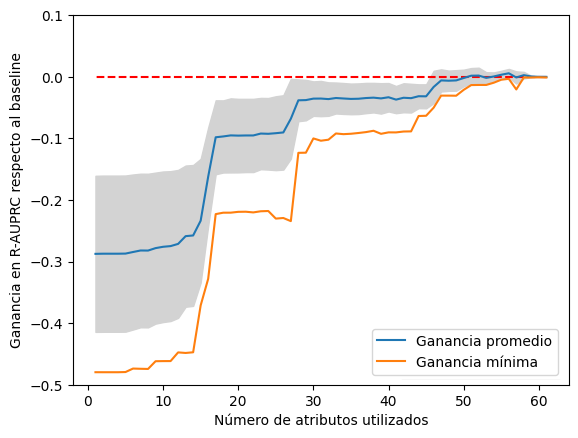
\includegraphics[width=0.49\textwidth]{Kap6/pearson_linear_CORRELATIONS_BIG_PICTURE.png} &   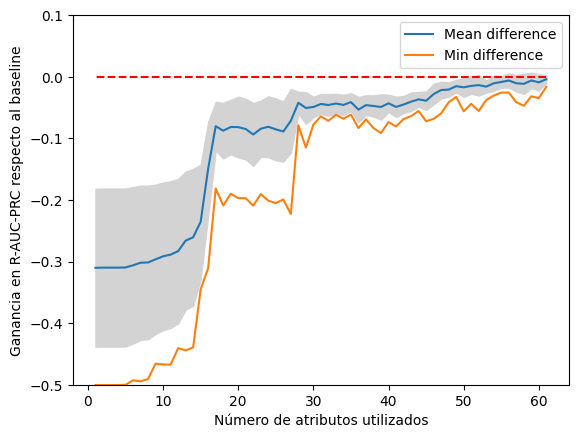
\includegraphics[width=0.49\textwidth]{Kap6/pearson_rbf_CORRELATIONS_BIG_PICTURE.png} \\
(a) SVM-Lineal & (b) SVM-RBF
\end{tabular}
\caption{Estas gráficas permiten apreciar la diferencia en R-AUPRC respecto a la base de referencia, obtenida al realizar utilizar los $k$ atributos menos correlacionados. Dado que esta diferencia se computó sobre 8 pares de tiles, para cada $k$ se muestra la media, la desviación estándar y el mínimo valor de entre todos los pares testeados. }
\label{fig:svm_correlation_summary}
\end{figure}

\section{Distribuciones de probabilidad subyacentes}

\subsection{ Histogramas de frecuencia }
En esta última sección simplemente se intentará comprender la distribución de probabilidad subyacente a cada uno de los atributos que estamos utilizando para describir RRLs. En la figura \ref{fig:distribuciones} podemos ver histogramas de frecuencia de los datos sin preprocesamiento alguno, en el tile b278. Dado el inmenso tamaño de cada tile (aprox. 500000 elementos cada uno), podemos asumir que estos histogramas son una buena aproximación de la distribución de probabilidad subyacente. En el anexo \ref{anexob_distribuciones} se muestran las distribuciones correspondientes a los tiles b234, b261 y b360. \\

Se puede observar que varios de los atributos no están distribuidos de forma normal, de hecho algunos atributos tienen distribuciones algo peculiares. El preprocesamiento elegido en los capítulos anteriores, binning quantile, se encargará de transformar estas distribuciones originales en distribuciones uniformes. \\

Un punto clave a resaltar es que las distribuciones de probabilidad que rigen algunos atributos son \textit{significativamente} diferentes entre distintos tiles. En la figura \ref{fig:distribuciones_distintas} se muestran algunos ejemplos prominentes. 


\begin{figure}[h!]
  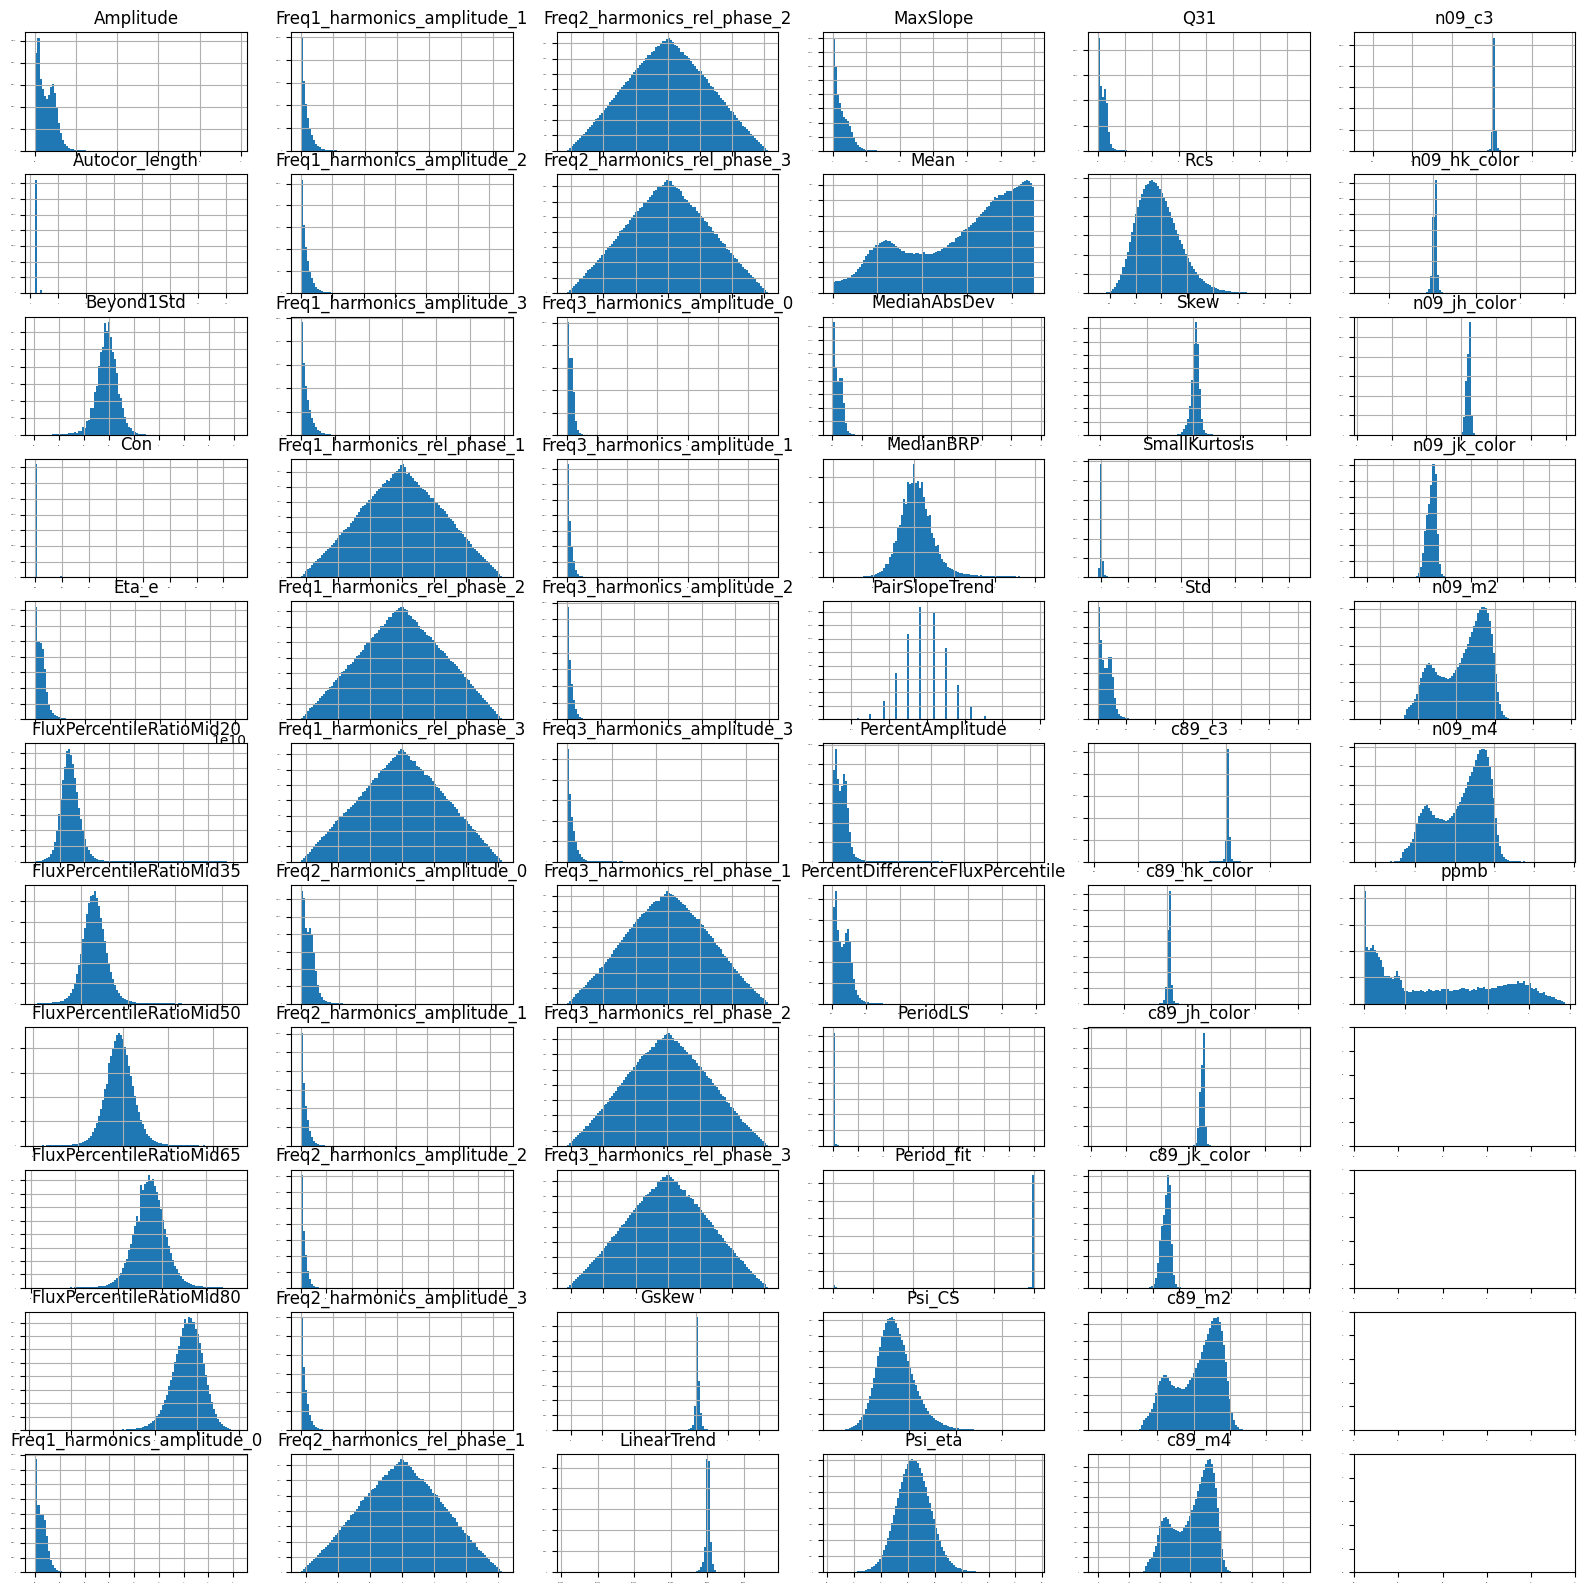
\includegraphics[width=\textwidth]{Kap6/allfeatures_b278.png}
\caption{Histogramas aproximando la distribución de probabilidad de cada atributo del tile b278.}
\label{fig:distribuciones}
\end{figure}

\begin{figure}[h!]
\begin{tabular}{cc}

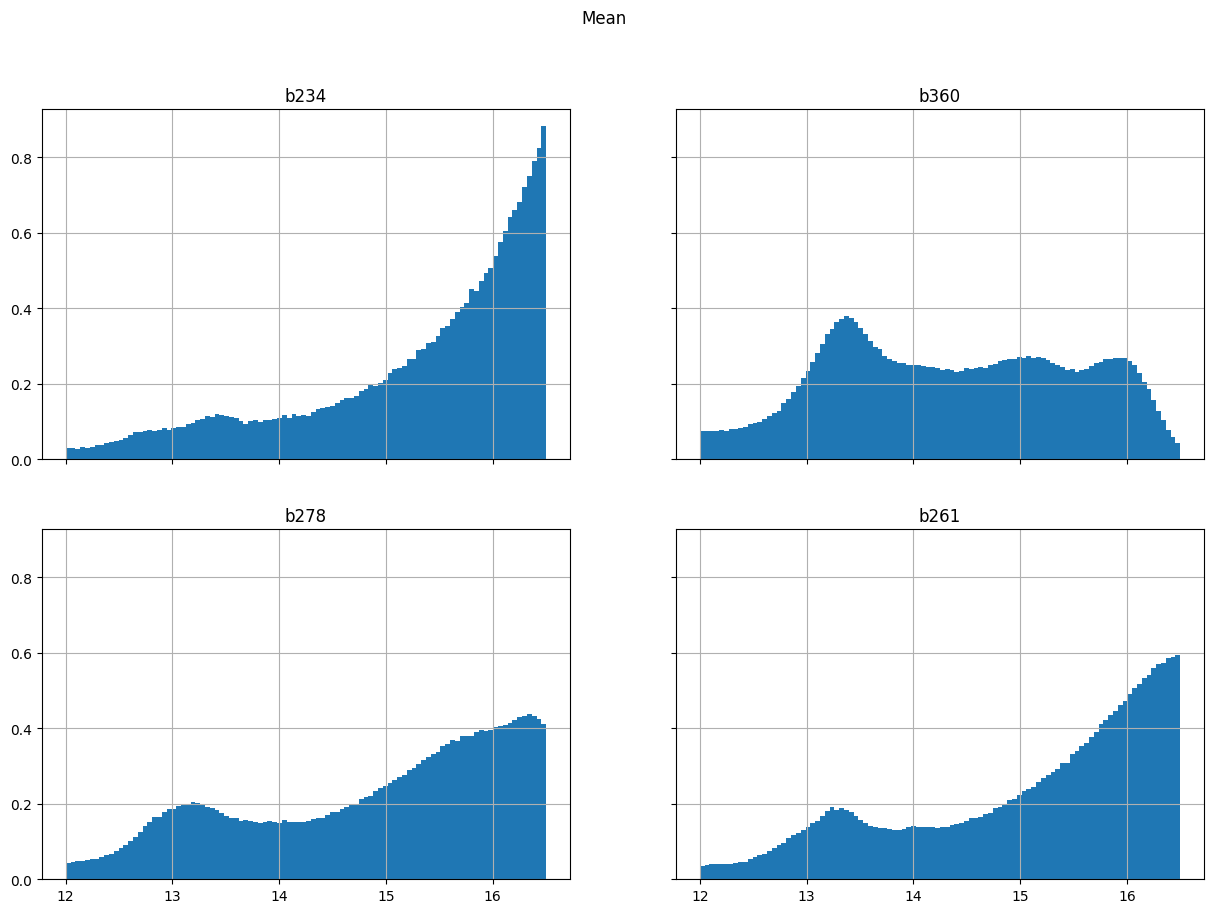
\includegraphics[width=0.49\textwidth]{Kap6/features/feature_comparison_34.png} & 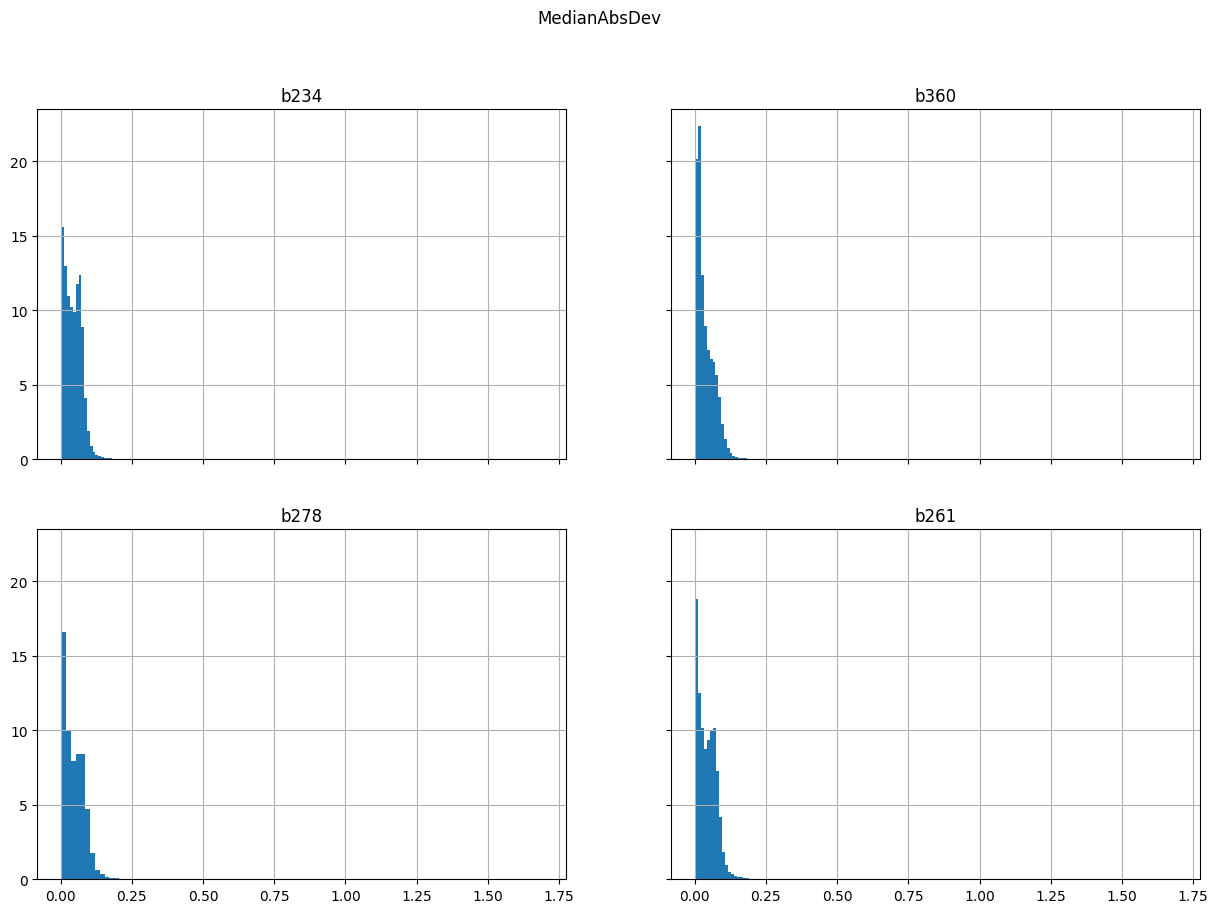
\includegraphics[width=0.49\textwidth]{Kap6/features/feature_comparison_35.png}  \\

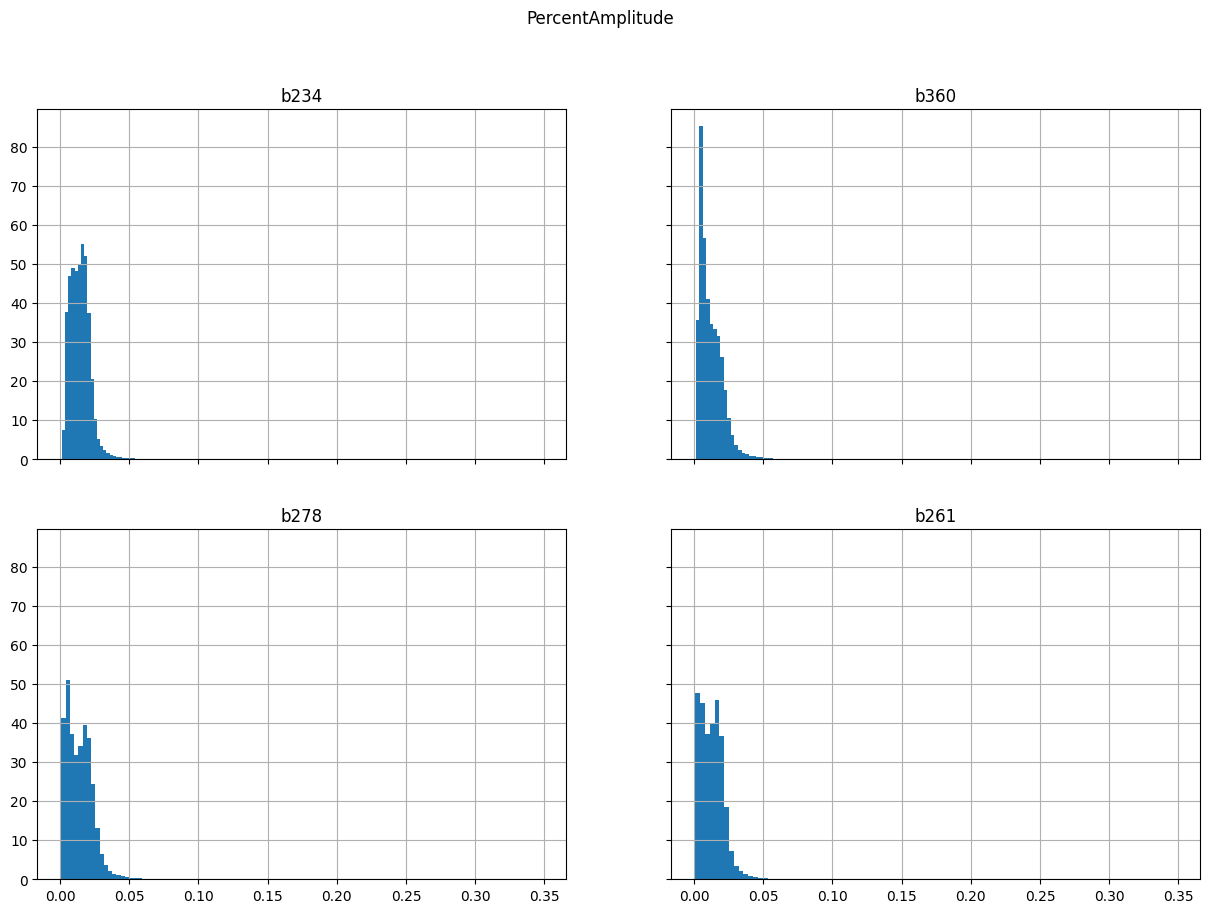
\includegraphics[width=0.49\textwidth]{Kap6/features/feature_comparison_38.png}  & 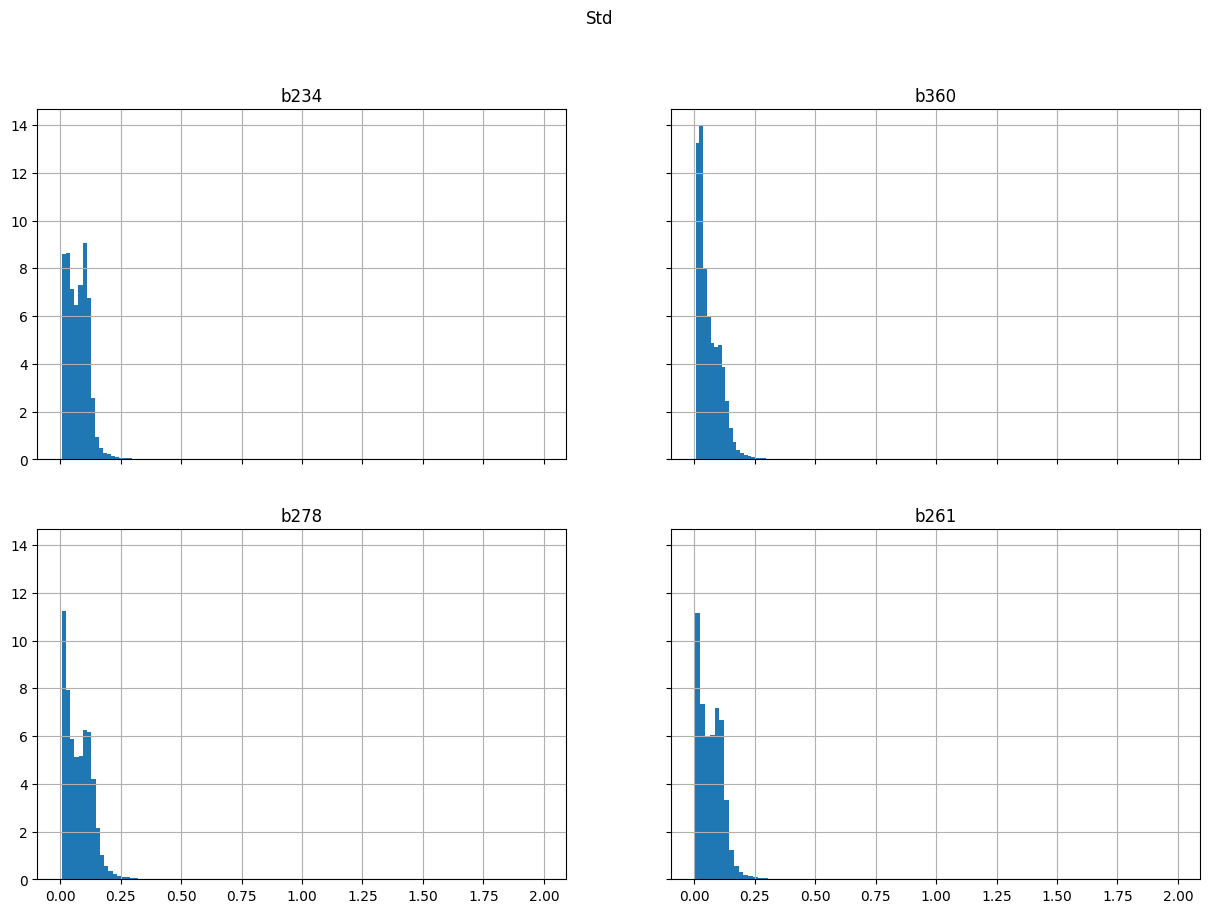
\includegraphics[width=0.49\textwidth]{Kap6/features/feature_comparison_48.png}  \\

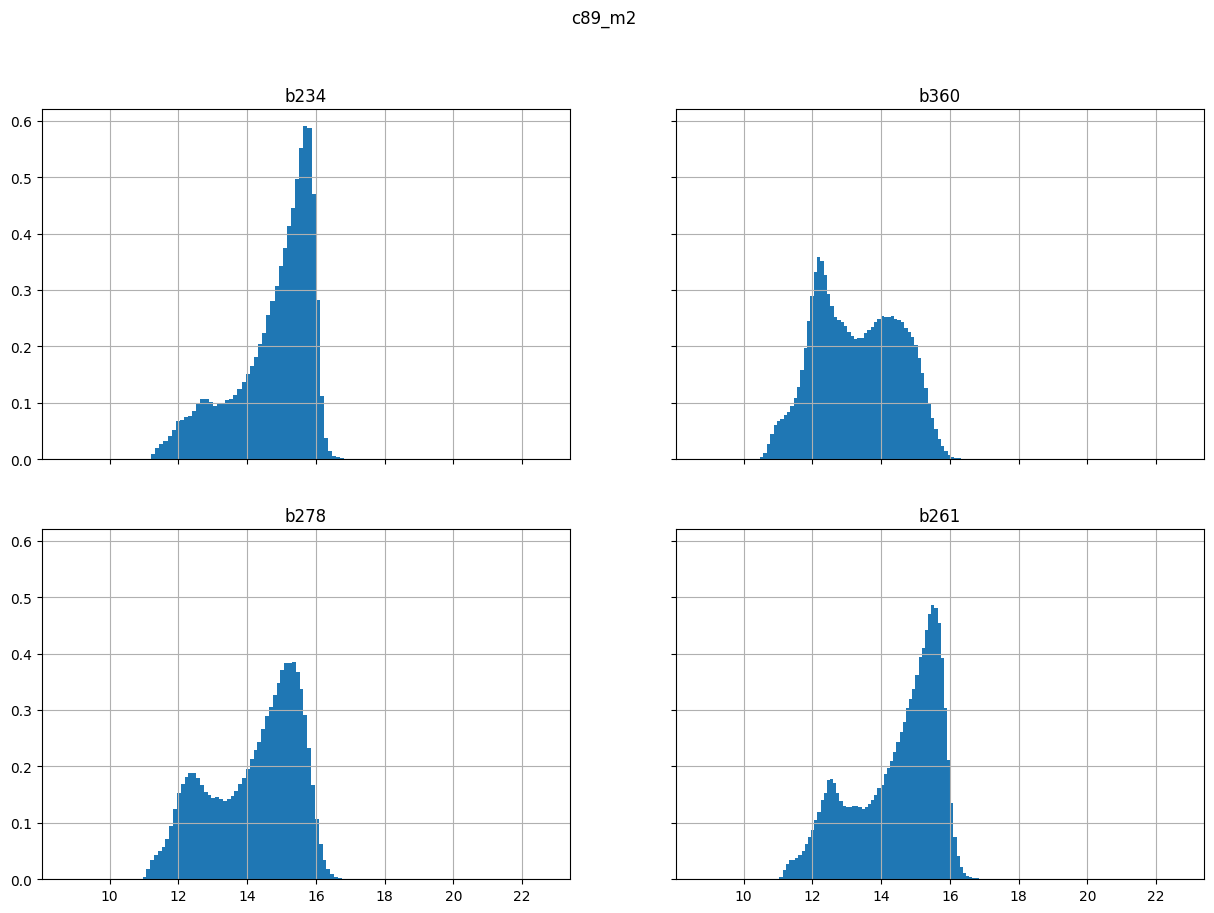
\includegraphics[width=0.49\textwidth]{Kap6/features/feature_comparison_53.png}   & 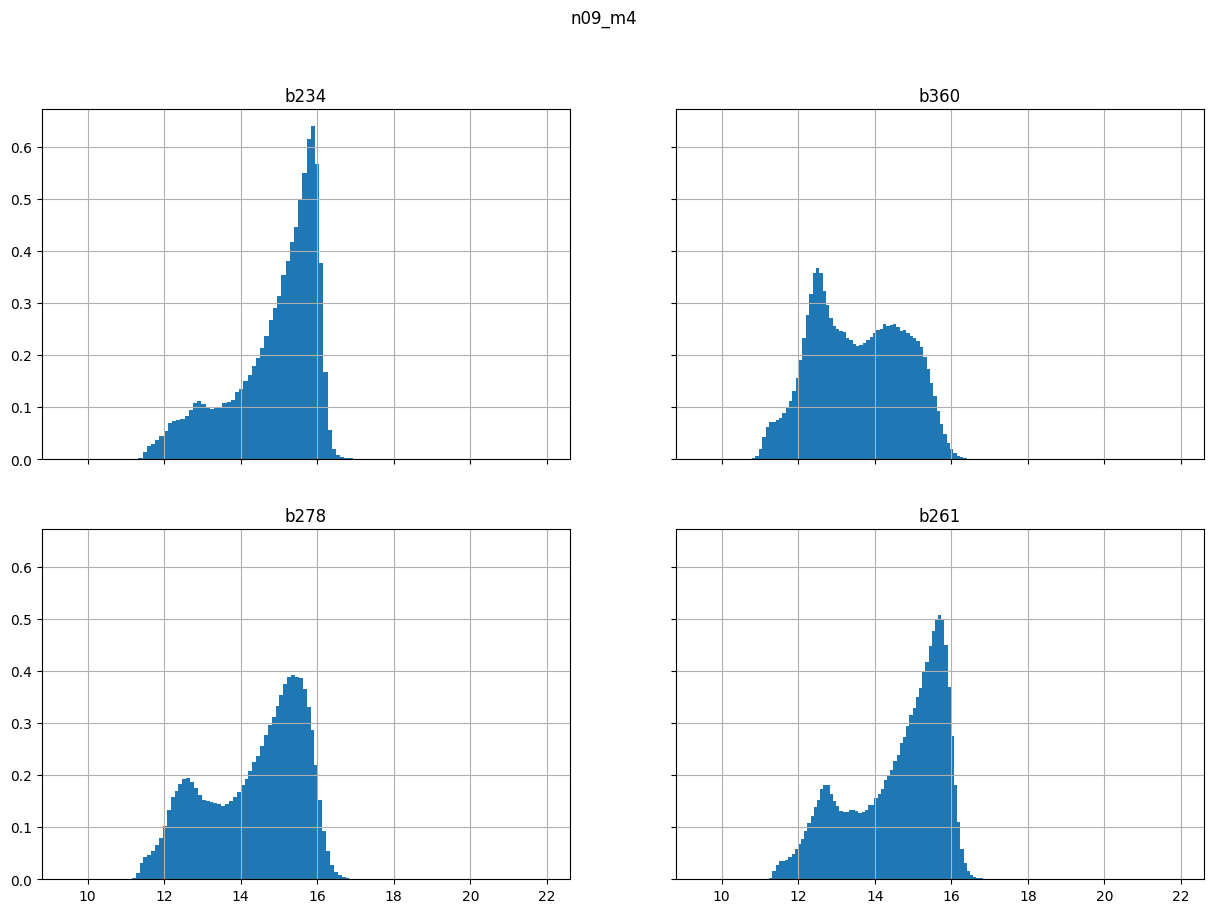
\includegraphics[width=0.49\textwidth]{Kap6/features/feature_comparison_60.png}  
\end{tabular}
\caption{En esta figura se grafican las distribuciones de probabilidad de algunos atributos que exhiben una notable diferencia entre distintos tiles. }
\label{fig:distribuciones_distintas}
\end{figure}

\subsection{Análisis de distribuciones}
\label{analisis_distribuciones}
Se ha observado que las distribuciones de probabilidad subyacentes a cada tile son diferentes entre sí, dado que la enorme cantidad de instancias de cada tile nos garantiza que las diferencias no son por chance. Esto podría representar un gran problema para SVM por dos motivos:

\begin{itemize}
\item La performance de SVM es altamente dependiente de la elección de hiperparámetros $C$ y $\gamma$. Dado que hemos seleccionado valores para estos hiperparémtros realizando cross validation en b278, existe la posibilidad de que tales valores no generalicen muy bien al entrenar y testear con otros tiles, cuya distribución de probabilidad puede ser distinta. Lo mismo aplica a otros hiperparámetros que hemos hallado en capítulos anteriores: número de bins, atributos a eliminar en selección de variables, etcétera.
\item El hiperplano separador hallado al entrenar SVM con un cierto tile puede no generalizar muy bien al testear con otro tile cuya distribución de probabilidad es distinta.
\end{itemize}

Ambas ideas se exploran en detalle en el capítulo \ref{variabilidad}. 

\section{Conclusiones}

En este capítulo hemos descubierto, mediante el uso de tests estadísticos, cuáles son los atributos de nuestro dataset que parecen no ser relevantes a la hora de distinguir RRLs. También hemos descubierto, mediante el uso de los mismos tests estadísticos y el índice Gini de RF que ciertos atributos, como PeriodFit y Psi\_CS, contienen información muy valiosa para detectar RRLs. SVM lineal falla en reconocer la importancia de tales atributos. \\

Se determinó que ciertos atributos de nuestros datasets presentan altas correlaciones monotónicas. Sin embargo, la inclusión de estos atributos no tiene un efecto perjudicial en la performance de SVM. \\

Finalmente, se concluyó que las distribuciones de probabilidad subyacentes a los distintos tiles son inherentemente distintas. Esto podría traer mayores problemas para SVM que para RF, tales como dificultad de escoger hiperparámetros que generalicen bien entre distintos tiles. Esta última hipótesis se estudiará en mayor profundidad en el capítulo \ref{variabilidad}.\\


